\section{Planteamiento del Problema}
El rendimiento es uno de los factores más influyentes en la experiencia del usuario al interactuar con software. Consiste principalmente en el tiempo que necesita el programa para responder a algún estímulo o el tiempo que necesita para ejecutar una o varias acciones. Un tiempo de respuesta del programa muy largo puede presentar una molestia al utilizar el programa. Según \ref{bib5}, existen 3 tiempos límites principales a tener en cuenta cuando se habla de desempeño de software:

\begin{enumerate}
    \item 0.1 segundo es el límite para hacer sentir al usuario que el programa está reaccionando instantáneamente.
    \item 1 segundo es el límite para no interrumpir el flujo de trabajo del usuario.
    \item 10 segundos es el límite para mantener la concentración del usuario, si se tiene un tiempo de respuesta mayor a este, el usuario perderá interés en la aplicación.
\end{enumerate}

El rendimiento puede ser incrementado mediante la sustitución de elementos de Hardware por otros con mayores capacidades de procesamiento. Sin embargo, debido a los costos adicionales que esto puede conllevar, es preferible hacer uso de la optimización del Software para mejorar el rendimiento del mismo. La optimización del Software consiste en rediseñar el Software de tal manera que tenga el mismo propósito de antes, sin embargo, que lo logre de una manera más eficiente ya sea necesitando menor espacio temporal en memoria o necesitando una menor cantidad de tiempo para hacer sus operaciones. Uno de los métodos más comunes para la optimización de programas es la división de un problema grande en problemas más pequeños que requieren menos esfuerzo para resolverse. Lo anterior corresponde a la expresión "Divide y vencerás" y en ciencias de la computación frecuentemente se implementa mediante funciones recursivas, las cuales son una forma de diseñar bucles definiendo funciones que se llaman a si mismas hasta que se cumple una condición. Lo anterior se puede utilizar cuando se tienen conjuntos de datos de gran tamaño para analizar ya que permite descartar la mayoría de los datos y solamente analizar un conjunto pequeño. La aplicación más simple de esta forma de optimización es en los algoritmos de búsqueda. El algoritmo de búsqueda lineal recorre todo un arreglo para intentar encontrar un elemento dentro de este. En la figura 1 se puede ver el algoritmo de búsqueda lineal.
\begin{figure}[!htbp]
    \centering
    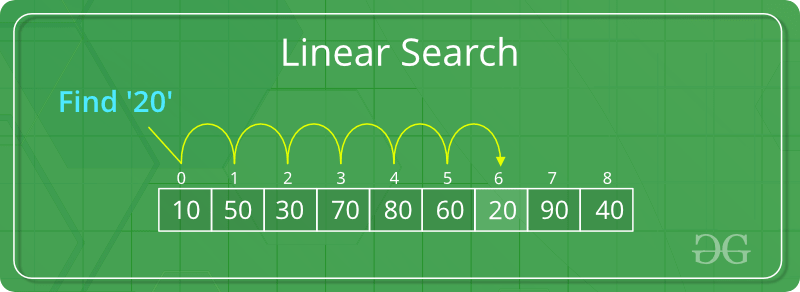
\includegraphics[width=.6\textwidth,height=.3\textwidth]{figures/linear_search.png}
    \caption{Búsqueda lineal \ref{bib6}}
    \label{fig:my_label}
\end{figure}
El rendimiento del algoritmo de búsqueda lineal depende de la posición del elemento que se va a buscar. Si este está en el inicio de la lista, lo encontrará inmediatamente, sin embargo, si este está al final de la lista tendrá que recorrerla toda para encontrar al elemento. En listas de gran tamaño esto significa que el algoritmo puede tomarse una gran cantidad de tiempo. El algoritmo de búsqueda binaria es otro algoritmo de búsqueda que necesita que los elementos de entrada estén ordenados, este algoritmo compara con el elemento central de la lista y si este es menor al elemento que se busca, lo descarta junto con la mitad inferior de la lista, si es mayor, descarta la mitad superior. El algoritmo continúa en la mitad que no se decartó hasta que se encuentre el elemento que se busca. El hecho de que se descarte la mitad de la lista con cada iteración aumenta la velocidad del algoritmo especialmente cuando la lista tiene un tamaño muy grande. En la figura 2 se puede ver el algoritmo de búsqueda binaria.
\begin{figure}[!htbp]
    \centering
    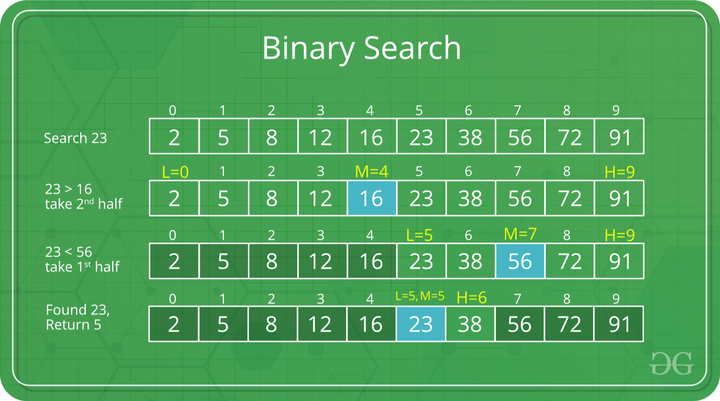
\includegraphics[width=.6\textwidth,height=.4\textwidth]{figures/binary_search.png}
    \caption{Búsqueda binaria \ref{bib7}}
    \label{fig:my_label}
\end{figure}